\chapter{Implementierung}%

\label{cha:Implementierung}
%was man alles anpassen muss

\colorbox{red!30}{DQN Algoritmus zum lernen des Spiels}\\



Es wurde sich für eine bestehende grundlegende Implementierung entschieden welche schon die Spiellogik von Vier Gewinnt sowie einen sehr einfachen Reinforcement Learning Ansatz enthält. In dieser Version lernt der Agent gegen einen Gegner zu gewinnen der zufällige Züge macht.\\
Diese Implentierung wurde um einen Gegner erweitert der seine Züge nach dem Minimax Algorithmus auswählt.\\
Weitergehend wurde die reinforcement learning Implementierung überarbeitet um gegen den Minimax Algorithmus gewinnen zu können.\\
Diese Implementierungen werden hier einmal genauer beschrieben:\\

\section{Minimax}
Der Minimax Algorithmus wurde als Teil des Environments implementiert und besteht im Groben aus zwei Teilen. Einmal die Funktion $check\_next\_actions$ die den Suchbaum für die nächsten Züge aufbaut. Und die Funktion $find\_best\_move$ die den Suchbaum nach dem besten Zug durchsucht.

\subsection{check\_next\_actions}
Das erstellen des Suchbaums funktioniert nach dem Negamax Algorithmus, es wird also eine Funktion für beide Spieler genutzt und immer abwechselnd das Maximum und das Minimum gesucht.

\subsection{find\_best\_move}
Das Suchen des besten Zuges wird durch die Alpha-Beta Suche beschleunigt indem bestimmte Äste des Suchbaumes, die sicher nicht zum gewünschten besten Zug führen, nicht weiter betrachtet werden. Dazu wurde noch eine Funktion zur Wahrscheinlichkeitsverteilung Implementiert die dafür sorgt, dass der Minimax Algorithmus in bestimmten Situationen mit einer gewissen Chance nicht optimal spielt.

\subsection{Wahrscheinlichkeitsverteilung}
\colorbox{red!30}{TODO}

\section{Reinforcement Learning}

\colorbox{red!30}{TODO link}

\subsection{Environment}
In Vier Gewinnt ist dies das Spielfeld und der Gegner. Das Spielfeld ist hier ein zweidimensionales Array der Länge 6 * 7. Der Gegner ist während des Lernens ein Computergegner der nach dem Minimax Algorithmus handelt. \\
\colorbox{red!30}{Done?}

\subsection{Agent}
Der Agent ist einer der beiden Spieler von Vier Gewinnt, welcher lernt seine Züge durch die ihm gegebne Policy auszuwählen, um einen möglichst hohen Reward zu erhalten.\\
\colorbox{red!30}{Done?} 

\subsection{Policy}
Als Policy wurde sich für die Epsilon-Greedy Policy entschieden da dies sehr gut für DQNs Funktioniert. Epsilon-Greedy beschreibt das Verhalten des Agenten welches entweder explorativ oder ausbeutend ist. Ist das Verhalten explorativ entscheidet sich der Agent für einen Zug den er vorher noch nicht oder selten gemacht hat um diesen zu erlernen. Ist das Verhalten ausbeutend so wird der Zug genommen welcher derzeitig die höchste Gewinnchance bietet. Zum Anfang des Lernens macht es natürlich Sinn, dass der Agent ganz viel erkundet da er noch kein Wissen über das Spiel besitzt. Hat der Agent dann einige Spiele hinter sich kann er auf die ausbeutende Strategie umschalten. Um dieses Verhalten des erstigen Erkundens und späteren Ausbeutens zu ermöglichen nutzt die Epsilon-Greedy Policy die Formel: $np.random.rand())<1-\epsilon$. Gibt diese Formel Wahr zurück so wird erkundet, gibt sie Falsch aus wird ausgebeutet. Der Wert von Epsilon ist am Anfang etwas mehr als Null und wird wärend der Lernphase langsam erhöht bis er etwas weniger als 1 erreicht hat. Somit ist das Ergebniss der Formel am Anfang meistens Wahr und später meistens Falsch.

\subsection{State}
 Für Vier Gewinnt beschreibt der State welche der 42 Felder mit welchen Steinen befüllt sind. Ein Beispiel für so einen State kann man in dem Abschnitt \hyperref[sec:visualisierung]{Visualsierung des Spiels} finden.\\
\colorbox{red!30}{Done?}

\subsection{Actions}
Die Actions in Vier Gewinnt beschreiben die sieben Löcher in die der Agent Steine werfen kann.\\
\colorbox{red!30}{Done?} 

\subsection{Reward}
 Zuerst wurde eine einfache diskrete Implementierung erstellt welche den Reward immer zum Ende einer Partie ausgibt, wobei dieser beim Gewinn 1 beim Verlieren -1 und wenn die Partie unentschieden ausgeht 0 beträgt.
Dies wurde durch die Anzahl der Züge um eine kontinuierliche Komponente erweitert. Hierfür wird der Reward der durch die diskrete Implementierung ermittelt wurde durch die Anzahl der Züge geteilt. Da es nicht möglich ist vor dem vierten Zug zu gewinnen wird erst ab diesem Zug gezählt. Es ergibt sich also die Formel: $$\frac{Reward}{Anzahl Züge-3}$$.
Wie man in \colorbox{red!30}{TODO Bild von der Rewardkurve} gut sehen kann wird somit das schnelle Gewinnen mehr belohnt und das schnelle Verlieren mehr bestraft. \\

\colorbox{red!30}{TODO credit assignment problem (bewertung nur am ende)}\\

\subsection{Q-Funktion}
\colorbox{red!30}{TODO} %ausführen

\section{Lernen vom Gegner}
Um das Lernen des Agenten zu verbessern wurde sich dazu entschieden, dass der Agent auch die Züge seines Gegners zum lernen nutzen kann. Dies ist für Vier Gewinnt erlaubt, da es sich um ein Spiel mit perfekter Information handelt. Es sind also jedem Spieler zum Zeitpunkt einer Entscheidung alle Informationen über das Spiel ersichtlich. Da ein menschlicher Anfänger in diesem Spiel, bei einer Niederlage an den Spielzügen seines Gegners lernen kann, wurde dies auch als sinnvoll für den Agenten angesehen. Um diese Informationen aufnehmen zu können wurden die Daten über das aktuelle Spielfeld und den gemachten Zug angepasst. Hierfür wird das gesammte Spiel einen halben Zug in der Vergangenheit betrachtet. Das heißt der Agent versetzt sich in die Rolle seines Gegners. Da der Agent weiß welche Zug sein Gegner gemacht hat kann er somit das negierte Spielfeld als Startzustand und den Zug seines Gegners als Aktion nutzen. 

\section{Graphische Darstellung}
Um die Effektivität der verschiedenen Versionen zu vergleichen wird der Reward in einem Graphen geplottet. Dies wird mit dem Paket pyplot von matplotlib gemacht.\\
\colorbox{red!30}{TODO Beispiel wenn es existiert}

\section{Visualsierung des Spiels}
\label{sec:visualisierung}
Da das Spielfeld im Code nur als zweidimensionales Array,welches mit 1, 0 und -1 gefüllt ist, existiert ist es für den Menschen nicht so einfach zu erkennen was gerade im Spiel passiert ist. Hierfür wurde mit Hilfe des Python Pakets colorama eine Visualisierung erschaffen. Diese wandelt alle Felder in den Unicode Character 'BLACK CIRCLE' (U+25CF) um wobei die 1 Gelb und die -1 Rot eingefärbt werden. Hierzu wird noch der Hintergrund Blau eingefärbt um dem Design des Spiels möglichst nah zu kommen. \\
Abbildung \ref{fig:spielfeld_konsole} ist ein durch diese Weise erstelltes Spielfeld für das Interne Array:
$$[[ 0  0  0  0  0  0  0]
 [ 0  0  0  0  0  0  0]
 [ 0  0  0  0  0 -1  0]
 [ 0  0  0  0  0 -1  0]
 [ 1  0  1 -1  0 -1  0]
 [ 1  1 -1  1  0 -1  1]]$$\\

\begin{figure}[h!]
  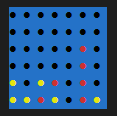
\includegraphics[width=117px,height=116px]{spielfeld_konsole.png}
  \centering
  \caption{Das Spielfeld auf der Konsole}
  \label{fig:spielfeld_konsole}
\end{figure}
